\documentclass[../main.tex]{subfiles}
\begin{document}
	\chapter{A generalized element concept}
	\label{chap:chap_6}
	\noindent So far, finite element computing has employed the nodes and element lists
	together with the definition of the basis functions in the reference element.
	
	Suppose we want to introduce a piecewise constant approximation with one basis function $\tilde{\varphi}_{0}(x)=1$ in the reference element, corresponding to a $\varphi_{i}(x)$ function that is 1 on element number $i$ and zero on all other elements. Although we could associate the function value with a node in the middle of the elements, there are no nodes at the ends, and the previous code snippets will not work because we cannot find the element boundaries from the nodes list.
	\section[Cells, vertices, and degrees of freedom]{Cells, vertices, and degrees of freedom}
	\label{sec:sec_6_1}
	We now introduce \textit{cells} as the subdomains $\Omega^{(e)}$ previously referred as elements. The cell boundaries are denoted as \textit{vertices}. The reason for this name is that cells are recognized by their vertices in $2 \mathrm{D}$ and 3D. We also define a \textit{set of degrees of freedom}, which are the quantities we aim to compute. The most common type of degree of freedom is the value of the unknown function $u$ at some point. (For example, we can introduce nodes as before and say the degrees of freedom are the values of $u$ at the nodes.) The basis functions are constructed so that they equal unity for one particular degree of freedom and zero for the rest. This property ensures that when we evaluate $u=\sum_{j} c_{j} \varphi_{j}$ for degree of freedom number $i$, we get $u=c_{i}$. Integrals are performed over cells, usually by mapping the cell of interest to a \textit{reference cell}.
	
	With the concepts of cells, vertices, and degrees of freedom we increase the decoupling of the geometry (cell, vertices) from the space of basis functions. We will associate different sets of basis functions with a cell. In 1D, all cells are intervals, while in 2D we can have cells that are triangles with straight sides, or any polygon, or in fact any two-dimensional geometry. Triangles and quadrilaterals are most common, though. The popular cell types in $3 \mathrm{D}$ are tetrahedra and hexahedra.
	\section[Extended finite element concept]{Extended finite element concept}
	\label{sec:sec_6_2}
	The concept of a finite element is now
	\begin{itemize}
		\item a \textit{reference cell} in a local reference coordinate system;
		\item a set of \textit{basis functions} $\tilde{\varphi}_{i}$ defined on the cell;
		\item a set of \textit{degrees of freedom} that uniquely determines the basis functions such that $\tilde{\rho}_{i}=1$ for degree of freedom number $i$ and $\tilde{\rho}_{i}=0$ for all other degrees of freedom;
		\item a mapping between local and global degree of freedom numbers, here called the \textit{dof map};
		\item a geometric \textit{mapping} of the reference cell onto to cell in the physical domain.
	\end{itemize}
	There must be a geometric description of a cell. This is trivial in 1D since the
	cell is an interval and is described by the interval limits, here called vertices. If the cell is $\Omega^{(e)}=\left[x_{L}, x_{R}\right]$, vertex 0 is $x_{L}$ and vertex 1 is $x_{R}$. The reference cell in $1 \mathrm{D}$ is $[-1,1]$ in the reference coordinate system $X$.
	The expansion of $u$ over one cell is often used:
	\begin{equation}\label{eqa92}
		u(x)=\tilde{u}(X)=\sum_{r} c_{r} \tilde{\rho}_{r}(X), \quad x \in \Omega^{(e)}, X \in[-1,1],
	\end{equation}
	where the sum is taken over the numbers of the degrees of freedom and $c_{r}$ is the value of $u$ for degree of freedom number $r$.
	
	Our previous $\mathrm{P} 1, \mathrm{P} 2$, etc., elements are defined by introducing $d+1$ equally spaced nodes in the reference cell and saying that the degrees of freedom are the $d+1$ function values at these nodes. The basis functions must be 1 at one node and 0 at the others, and the Lagrange polynomials have exactly this property. The nodes can be numbered from left to right with associated degrees of freedom that are numbered in the same way. The degree of freedom mapping becomes what was previously represented by the elements lists. The cell mapping is the same affine mapping (\hyperref[eqa61]{61}) as before.
	\section[Implementation]{Implementation}
	\label{sec:sec_6_3}
	\noindent Implementationwise,
	\begin{itemize}
		\item we replace \mycode{nodes} by vertices;
		\item we introduce \mycode{cells} such that \mycode{cell [e] [r]} gives the mapping from local vertex $r$ in cell e to the global vertex number in vertices;
		\item we replace \mycode{elements} by \mycode{dof\textunderscore map} (the contents are the same for $\mathrm{P} d$ elements).
	\end{itemize}
	
	\noindent Consider the example from Section \hyperref[sec:sec_3_1]{3.1} where $\Omega=[0,1]$ is divided into two cells, $\Omega^{(0)}=[0,0.4]$ and $\Omega^{(1)}=[0.4,1]$, as depicted in Figure \hyperref[fig:img_16]{16} . The vertices are $[0,0.4,1]$. Local vertex 0 and 1 are 0 and $0.4$ in cell 0 and $0.4$ and 1 in cell 1 . A P2 element means that the degrees of freedom are the value of $u$ at three equally spacèd points (nodes) in each céll. The data structuress become
	\begin{lstlisting}[numbers=none]
		vertices = [0, 0.4, 1]
		cells = [[0, 1], [1, 2]]
		dof_map = [[0, 1, 2], [2, 3, 4]]	
	\end{lstlisting}
	If we would approximate $f$ by piecewise constants, known as $\mathrm{P} 0$ elements, we simply introduce one point or node in an element, preferably $X=0$, and define one degree of freedom, which is the function value at this node. Moreover, we set $\tilde{\varphi}_{0}(X)=1$. The \mycode{cells} and \mycode{vertices} arrays remain the same, but \mycode{dof\textunderscore map} is altered:
	\begin{lstlisting}[numbers=none]
		dof_map = [[0], [1]]	
	\end{lstlisting}
	We use the \mycode{cells} and \mycode{vertices} lists to retrieve information on the geometry of a cell, while \mycode{dof\textunderscore map}  is the $q(e, r)$ mapping introduced earlier in the assembly of element matrices and vectors. For example, the \mycode{Omega\textunderscore e}  variable (representing the cell interval) in previous code snippets must now be computed as
	\begin{lstlisting}[numbers=none]
		Omega_e = [vertices[cells[e][0], vertices[cells[e][1]]	
	\end{lstlisting}
	The assembly is done by
	\begin{lstlisting}[numbers=none]
		A[dof_map[e][r], dof_map[e][s]] += A_e[r,s]
		b[dof_map[e][r]] += b_e[r]	
	\end{lstlisting}
	We will hereafter drop the nodes and elements arrays and work exculsively
	with cells, vertices, and dof\textunderscore map. The module \textbf{fe\textunderscore approx1D\textunderscore numint.py} 
	now replaces the module \textbf{fe\textunderscore approx1D}  and offers similar functions that work
	with the new concepts:
	\begin{lstlisting}[numbers=none]
		from fe_approx1D_numint import *
		x = sp.Symbol('x')
		f = x*(1 - x)
		N_e = 10
		vertices, cells, dof_map = mesh_uniform(N_e, d=3, Omega=[0,1])
		phi = [basis(len(dof_map[e])-1) for e in range(N_e)]
		A, b = assemble(vertices, cells, dof_map, phi, f)
		c = np.linalg.solve(A, b)
		# Make very fine mesh and sample u(x) on this mesh for plotting
		x_u, u = u_glob(c, vertices, cells, dof_map, resolution_per_element=51)
		plot(x_u, u)	
	\end{lstlisting}
	These steps are offered in the \mycode{approximate} function, which we here apply to see
	how well four P0 elements (piecewise constants) can approximate a parabola:
	\begin{lstlisting}[numbers=none]
		from fe_approx1D_numint import *
		x=sp.Symbol("x")
		for N_e in 4, 8:
			approximate(x*(1-x), d=0, N_e=N_e, Omega=[0,1])	
	\end{lstlisting}
	Figure \hyperref[fig:img_32]{32} shows the result.
	
	\section[Computing the error of the approximation]{Computing the error of the approximation}
	\label{sec:sec_6_4}
	So far we have focused on computing the coefficients $c_{j}$ in the approximation $u(x)=\sum_{j} c_{j} \varphi_{j}$ as well as on plotting $u$ and $f$ for visual comparison. A more quantitative comparison needs to investigate the error $e(x)=f(x)-u(x)$. We mostly want a single number to reflect the error and use a norm for this purpose, usually the $L^{2}$ norm
	$$
	\|e\|_{L^{2}}=\left(\int_{\Omega} e^{2} d x\right)^{1 / 2}.
	$$
	\begin{figure}[H]
		\centering
		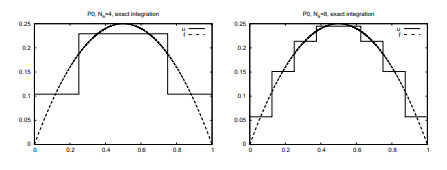
\includegraphics[width=0.7\linewidth]{img_32}
		\caption{Approximation of a parabola by 4 (left) and 8 (right) P0 elements.}
		\label{fig:img_32}
	\end{figure}
	\noindent Since the finite element approximation is defined for all $x \in \Omega$, and we are interested in how $u(x)$ deviates from $f(x)$ through all the elements, we can either integrate analytically or use an accurate numerical approximation. The latter is more convenient as it is a generally feasible and simple approach. The idea is to sample $e(x)$ at a large number of points in each element. The function u\textunderscore glob in the \textbf{fe\textunderscore approx1D\textunderscore numint}  module does this for $u(x)$ and returns an array $\mathbf{x}$ with coordinates and an array $u$ with the $u$ values:
	\begin{lstlisting}[numbers=none]
		x, u = u_glob(c, vertices, cells, dof_map,
		resolution_per_element=101)
		e = f(x) - u
	\end{lstlisting}
	Let us use the Trapezoidal method to approximate the integral. Because different
	elements may have different lengths, the x array has a non-uniformly distributed
	set of coordinates. Also, the \mycode{u\textunderscore glob}  function works in an element by element
	fashion such that coordinates at the boundaries between elements appear twice.
	We therefore need to use a ”raw” version of the Trapezoidal rule where we just
	add up all the trapezoids:
	$$
	\int_{\Omega} g(x) d x \approx \sum_{j=0}^{n-1} \frac{1}{2}\left(g\left(x_{j}\right)+g\left(x_{j+1}\right)\right)\left(x_{j+1}-x_{j}\right),
	$$
	if $x_{0}, \ldots, x_{n}$ are all the coordinates in $\mathrm{x}$. In vectorized Python code,
	\begin{lstlisting}[numbers=none]
		g_x = g(x)
		integral = 0.5*np.sum((g_x[:-1] + g_x[1:])*(x[1:] - x[:-1]))	
	\end{lstlisting}
	Computing the $L^{2}$ norm of the error, here named E, is now achieved by
	\begin{lstlisting}[numbers=none]
		e2 = e**2
		E = np.sqrt(0.5*np.sum((e2[:-1] + e2[1:])*(x[1:] - x[:-1]))	
	\end{lstlisting}
	\begin{mybox}
		\textbf{How does the error depend on $h$ and $d$ ?}
		
		\noindent Theory and experiments show that the least squares or projection/Galerkin method in combination with $\mathrm{P} d$ elements of equal length $h$ has an error
		\begin{equation}\label{eqa93}
			\|e\|_{L^{2}}=C h^{d+1},
		\end{equation}
		
		\noindent where $C$ is a constant depending on $f$, but not on $h$ or $d$.
	\end{mybox}
	
	\section[Example: Cubic Hermite polynomials]{Example: Cubic Hermite polynomials}
	\label{sec:sec_6_5}
	The finite elements considered so far represent u as piecewise polynomials with
	discontinuous derivatives at the cell boundaries. Sometimes it is desirable to
	have continuous derivatives. A primary examples is the solution of differential
	equations with fourth-order derivatives where standard finite element formulations lead to a need for basis functions with continuous first-order derivatives.
	The most common type of such basis functions in 1D is the so-called cubic
	Hermite polynomials. The construction of such polynomials, as explained next,
	will further exemplify the concepts of a cell, vertex, degree of freedom, and dof
	map.
	
	Given a reference cell $[-1,1]$, we seek cubic polynomials with the values of the \textit{function} and its \textit{first-order derivative} at $X=-1$ and $X=1$ as the four degrees of freedom. Let us number the degrees of freedom as
	\begin{itemize}
		\item 0 : value of function at $X=-1$
		\item 1: value of first derivative at $X=-1$
		\item 2: value of function at $X=1$
		\item 3: value of first derivative at $X=1$
	\end{itemize}
	By having the derivatives as unknowns, we ensure that the derivative of a basis function in two neighboring elements is the same at the node points.
	The four basis functions can be written in a general form
	$$
	\tilde{\varphi}_{i}(X)=\sum_{j=0}^{3} C_{i, j} X^{j},
	$$
	with four coefficients $C_{i, j}, j=0,1,2,3$, to be determined for each $i$. The constraints that basis function number $i$ must be 1 for degree of freedom number $i$ and zero for the other three degrees of freedom, gives four equations to determine $C_{i, j}$ for each $i$. In mathematical detail,
	$$
	\begin{aligned}
		\tilde{\varphi}_{0}(-1)=1, & \tilde{\varphi}_{0}(1)=\tilde{\varphi}_{0}^{\prime}(-1)=\tilde{\varphi}_{i}^{\prime}(1)=0, \\
		\tilde{\varphi}_{1}^{\prime}(-1)=1, & \tilde{\varphi}_{1}(-1)=\tilde{\varphi}_{1}(1)=\tilde{\varphi}_{1}^{\prime}(1)=0, \\
		\tilde{\varphi}_{2}(1)=1, & \tilde{\varphi}_{2}(-1)=\tilde{\varphi}_{2}^{\prime}(-1)=\tilde{\varphi}_{2}^{\prime}(1)=0, \\
		\tilde{\varphi}_{3}^{\prime}(1)=1, & \tilde{\varphi}_{3}(-1)=\tilde{\varphi}_{3}^{\prime}(-1)=\tilde{\varphi}_{3}(1)=0 .
	\end{aligned}
	$$
	These four $4 \times 4$ linear equations can be solved, yielding the following formulas for the cubic basis functions:
	\begin{equation}\label{eqa94}
		\tilde{\varphi}_{0}(X) =1-\frac{3}{4}(X+1)^{2}+\frac{1}{4}(X+1)^{3}
	\end{equation}
	\begin{equation}\label{eqa95}
		\tilde{\varphi}_{1}(X) =-(X+1)\left(1-\frac{1}{2}(X+1)\right)^{2}
	\end{equation}
	\begin{equation}\label{eqa96}
		\tilde{\varphi}_{2}(X) =\frac{3}{4}(X+1)^{2}-\frac{1}{2}(X+1)^{3}
	\end{equation}
	\begin{equation}\label{eqa97}
		\tilde{\varphi}_{3}(X) =-\frac{1}{2}(X+1)\left(\frac{1}{2}(X+1)^{2}-(X+1)\right)
	\end{equation}
	\begin{equation}\label{eqa98}
	\end{equation}	
	The construction of the dof map needs a scheme for numbering the global degrees of freedom. A natural left-to-right numbering has the function value at vertex $x_{i}$ as degree of freedom number $2 i$ and the value of the derivative at $x_{i}$ as degree of freedom number $2 i+1, i=0, \ldots, N_{e}+1$.
\clearpage
\end{document} 
